\documentclass{standalone}
\usepackage{tikz}
\usepackage{ctex,siunitx}
\setCJKmainfont{Noto Serif CJK SC}
\usepackage{tkz-euclide}
\usepackage{amsmath}
\usepackage{wasysym}
\usetikzlibrary{patterns, calc}
\usetikzlibrary {decorations.pathmorphing, decorations.pathreplacing, decorations.shapes,}
\begin{document}
\small
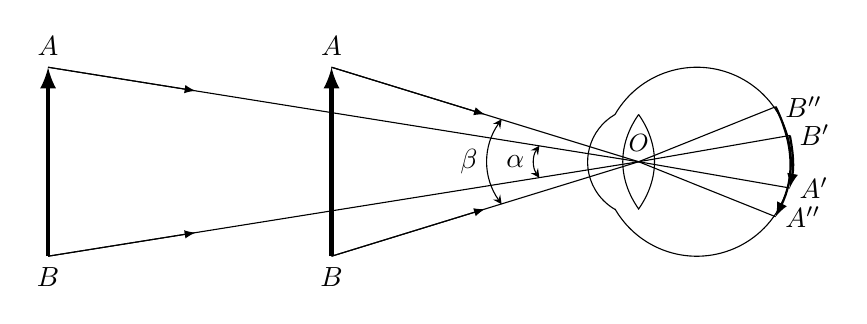
\begin{tikzpicture}[>=latex,scale=1.2]
  % eye begin
  \draw (0,.5) arc (150:-150:1);
  \draw (0,.5) arc (120:240:.58);
  \draw (0.25,.5)to [bend left=35] (.25,-.5)to [bend left=35](0.25,.5) ;
  % eye end
  \draw[->, ultra thick] (-6,-1)node[below]{$B$}--(-6,1)node[above]{$A$};
  \draw[->, ultra thick] (-3,-1)node[below]{$B$}--(-3,1)node[above]{$A$};
  \draw (-3,-1)--(0.25,0)--(1.7, .582)node[right]{$B''$};
  \draw (-3, 1)--(0.25,0)--(1.7, -.582)node[right]{$A''$};
  \draw (-6,-1)--(0.25,0)--(1.85, .278)node[right]{$B'$};
  \draw (-6,1)--(0.25,0)--(1.85, -.278)node[right]{$A'$};
  \draw [->, thick](1.7, .582)to [bend right=-26] (1.7, -.582);
  \draw [->,  thick](1.85, .278)to [bend right=-11] (1.85, -.278);
  \node at (0.25,0)[above]{\small $O$};
  \draw[->] (-3,-1)--(-2.75/2,-.5);
  \draw[->] (-3, 1)--(-2.75/2,.5);
  \draw[->] (-6,-1)--(-4.4375,-.75);
  \draw[->] (-6,1)--(-4.4375,.75);
  \draw [<->, >=stealth](-1.2, .45)to [bend left=-35]node[left]{$\beta$} (-1.2, -.45);
  \draw [<->, >=stealth](-.8, .17)to [bend left=-35]node[left]{$\alpha$} (-.8, -.17);
\end{tikzpicture}
\end{document}